% !TEX program = xelatex
\documentclass[10pt,letterpaper,twocolumn]{article}

\usepackage[top=0.72in,bottom=0.72in,left=0.72in,right=0.72in]{geometry}
\usepackage{fontspec}
\setmainfont{Latin Modern Roman}[
  Extension=.otf,UprightFont=lmroman10-regular,BoldFont=lmroman10-bold,
  ItalicFont=lmroman10-italic,BoldItalicFont=lmroman10-bolditalic]
\setsansfont{Latin Modern Sans}[
  Extension=.otf,UprightFont=lmsans10-regular,BoldFont=lmsans10-bold,
  ItalicFont=lmsans10-oblique,BoldItalicFont=lmsans10-boldoblique]
\setmonofont{Latin Modern Mono}[Extension=.otf,UprightFont=lmmono10-regular,Scale=0.82]

\usepackage{xcolor}
\usepackage{graphicx}
\usepackage{booktabs}
\usepackage{tabularx}
\usepackage{microtype}
\usepackage[numbers,sort&compress]{natbib}
\usepackage{titlesec}
\usepackage{enumitem}
\usepackage{fancyhdr}
\usepackage{hyperref}
\usepackage{xurl}
\usepackage[colorspec=0.92]{draftwatermark}
\usepackage{../ac-source-bundle}

\newfontfamily\acbold{ywft-processing-bold}[
  Path=../../system/public/type/webfonts/,Extension=.ttf]
\newfontfamily\aclight{ywft-processing-light}[
  Path=../../system/public/type/webfonts/,Extension=.ttf]
\definecolor{acpink}{RGB}{180,72,135}
\definecolor{acpurple}{RGB}{120,80,180}
\definecolor{acdark}{RGB}{64,56,74}
\definecolor{acgray}{RGB}{119,119,119}
\definecolor{draftcolor}{RGB}{180,72,135}
\renewcommand{\acsourcebundleblock}{%
  \IfFileExists{\jobname-source.zip}{%
    \par\vspace{0.35em}%
    \noindent\rule{\linewidth}{0.35pt}\par\vspace{0.18em}%
    \noindent{\small\bfseries\color{acpink}%
      \attachfile[color=0.706 0.282 0.529,icon=Paperclip,mimetype=application/zip,description={Machine-readable paper source bundle}]{\jobname-source.zip}%
      \hspace{0.45em}Source bundle}\par
    \vspace{0.12em}%
    \noindent{\scriptsize\color{acgray}%
      The attached ZIP contains the paper's machine-readable text sources and a plain-text inventory. It supports accessibility, audit, quotation, and reproducible editing; the PDF remains the canonical reading edition. Private evidence, credentials, raw datasets, generated PDFs, and unlisted assets are excluded.}\par
  }{}%
}
\DraftwatermarkOptions{text=WORKING DRAFT,fontsize=3cm,color=draftcolor!14,angle=45}
\titleformat{\section}{\normalfont\bfseries\normalsize\uppercase}{\thesection.}{0.5em}{}
\titlespacing{\section}{0pt}{0.9em}{0.2em}
\titleformat{\subsection}{\normalfont\bfseries\small}{\thesubsection}{0.5em}{}
\titlespacing{\subsection}{0pt}{0.55em}{0.12em}
\pagestyle{fancy}
\fancyhf{}
\renewcommand{\headrulewidth}{0pt}
\fancyfoot[C]{\footnotesize\thepage}
\setlist[itemize]{nosep,leftmargin=1.2em,itemsep=0.1em}
\setlist[enumerate]{nosep,leftmargin=1.4em,itemsep=0.1em}
\setlength{\parindent}{1em}
\setlength{\parskip}{0.18em}
\newcommand{\code}[1]{\nolinkurl{#1}}

\graphicspath{{figures/}{../arxiv-ac/figures/}{../arxiv-whistlegraph/figures/}}
\hypersetup{
  hidelinks,
  pdfauthor={@jeffrey},
  pdftitle={Three Kinds of Time: Arrangement Critique of lonerclub}}
\fancyhead[C]{\footnotesize\color{acpink}\textit{lonerclub --- arrangement critique}}
\setlength{\columnsep}{1.7em}
\tolerance=900
\emergencystretch=1em

\newcommand{\track}{\textit{lonerclub}}
\newcommand{\sourcework}{\textit{Loner}}
\newcommand{\dbfs}{\,dBFS}
\newcommand{\lufs}{\,LUFS}

\begin{document}

\twocolumn[{%
\begin{center}

\includegraphics[height=3.5em]{pals}\par\vspace{0.45em}
{\acbold\fontsize{25pt}{29pt}\selectfont\color{acdark} Three Kinds of Time}\par
\vspace{0.22em}
{\aclight\fontsize{12pt}{14pt}\selectfont\color{acpink}
  Arrangement critique of \track}\par
\vspace{0.35em}
{\small\color{acgray} Derived from \texttt{lonr} --- \sourcework{} (2021), composed and originally performed by Camille Klein}\par
\vspace{0.55em}
{\normalsize\href{https://prompt.ac/@jeffrey}{@jeffrey}}\par
{\small\color{acgray} Aesthetic.Computer / Whistlegraph Dot Org --- August 27, 2026}\par
{\small\color{acgray} ORCID: \href{https://orcid.org/0009-0007-4460-4913}{0009-0007-4460-4913}}\par
\vspace{0.35em}
{\small\color{acpurple}\url{https://aesthetic.computer}}\par
\vspace{0.55em}\rule{\textwidth}{1.5pt}\vspace{0.35em}
\end{center}

\begin{quote}
\small\noindent\textbf{Abstract.}
The 97.2-second \track{} release candidate already has a convincing form: Camille Klein's one-sentence whistlegraph is sung three times while a 122 BPM floor continues and the orchestra thickens. Its problem is narrower than ``needs a better arrangement.'' The three passes are differentiated mainly by accumulation. The middle pass is roughly 1\,dB RMS louder than either neighbor; detected onset density doubles from 4.2 to 8.0 events per second between the first two passes but stays flat in the third; and two transition rushes briefly move the spectral centroid from a 0.9--1.3\,kHz baseline toward 4\,kHz. They sound and measure as white-outs rather than hinges. The revision proposed here gives each pass one job: body, clock, club. It replaces each rush with a five-hit click figure, binds timbral events to specific lyric-marks, reserves low-frequency weight and reverberant width for the last pass, and keeps the direct vocal centered and continuous. The master already meets the studio's $-13.5$\,LUFS release law; the next improvement is arrangement, not more mastering.
\end{quote}
\vspace{0.4em}
}]

\section{One Sentence Is Enough Form}

\sourcework{} is one line: ``sitting curled up in myself, I think of a stone, just waiting very patiently for time to pass.'' Each lyric segment is also a drawn gesture~\cite{klein2021loner,scudder2026whistlegraph}. \track{} turns that 30-second score into a three-pass club record~\cite{whistlegraph2026lonerclub}. Repetition is therefore not a shortage of material. It is the material.

The release candidate's strongest decisions are already settled: the first sung word arrives at 0.84 seconds; the beat does not stop; the direct voice remains the narrative center; vocal arpeggiation has been removed; and the form ends after the third complete utterance rather than padding itself to a conventional runtime. The revision has one task: make each return of the sentence change the listener's relation to time.

The proposed reading is body (0:00--0:31.83), private time curled inward; clock (0:31.83--1:03.30), waiting made pulse; club (1:03.30--1:33.20), the room moving with her; and stamp (1:33.20--1:37.20), authorship after the sentence rather than a fourth act. That story is stronger than quiet / fuller / fullest because the difference survives without counting tracks.

\section{Project Context}

A whistlegraph binds visual, musical, and textual layers one-to-one: a sung phrase produces a drawn gesture, and the finished image is a score. Prior work describes the score as an interface rather than an illustration~\cite{scudder2026whistlegraph}. \track{} extends the form, so its arrangement should not merely accompany the source song; it should disclose the same structure at a larger timescale.

The studio doctrine is equally direct: composition is the arrangement of inspectable instruments, and a process that cannot be scored is not yet known~\cite{scudder2026compstrats}. Sampling is treated as a first-class authored object rather than opaque infrastructure~\cite{scudder2026sampling}. New layers therefore earn their place only when their role can be named.

\section{Method and Snapshot}

The critique fixes one reproducible object: \code{pop/loner/out/lonerclub-v4pid-release.wav}, modified 2026-08-27 10:41:54 EDT, SHA-256 \code{cfaed16556b4...d6bec7b0}. The stereo 48\,kHz master is 97.2 seconds. FFmpeg EBU R128 analysis reports $-13.5$\lufs{} integrated, 2.3\,LU loudness range, and $-3.2$\dbfs{} true peak.

The form was read against \code{wordclock.json}, the regulated 122 BPM note chart, the tracked C score, the release record, the active \code{neo:vod} arrangement history, and the rendered review-score timeline. The colocated analysis script measures RMS level, spectral centroid, onset strength, detected onset count, stereo correlation, and side/mid energy. These descriptors support the musical reading; they do not decide whether the music is good. This follows the rhythm platter's caution that a grid describes onset placement while groove remains a performed relation~\cite{scudder2026rhythmplatter}.

\begin{figure*}[t]
\centering
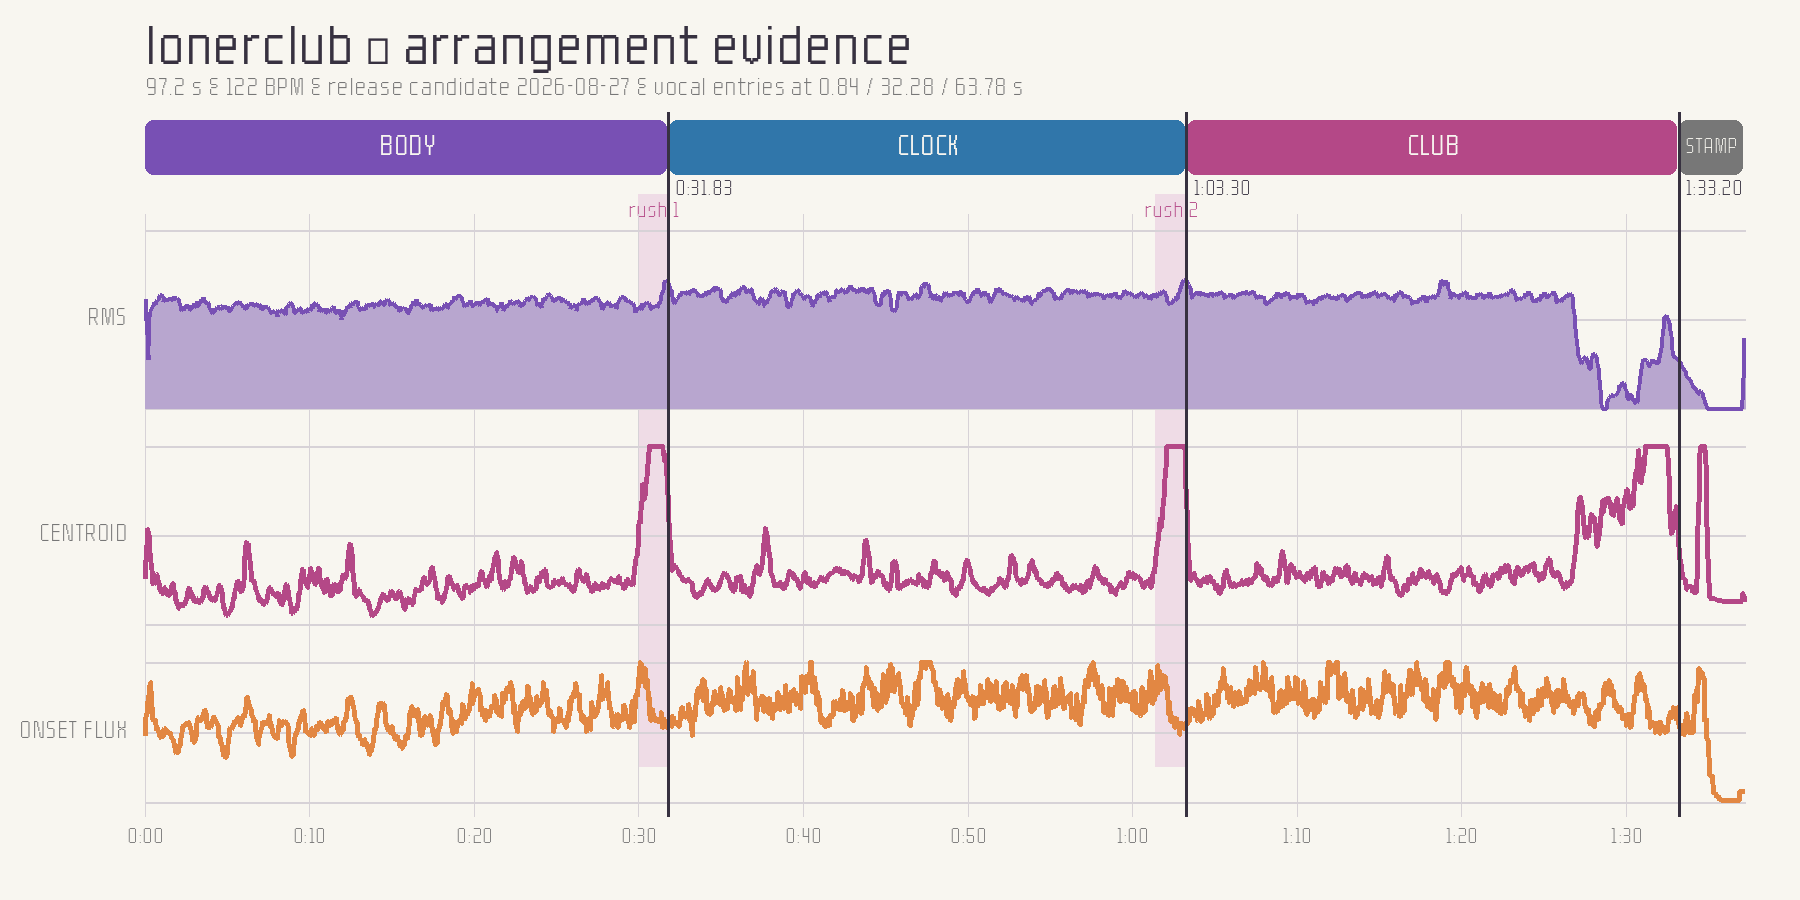
\includegraphics[width=\textwidth]{arrangement-evidence}
\caption{Arrangement-scale evidence from the fixed master. Energy remains nearly level through the three lyric passes. The second pass already carries the large onset-density increase; the third adds brightness rather than a new rhythmic rate. The two pink transition windows are broadband centroid spikes. Generated by the colocated \code{analysis.py}.}
\label{fig:evidence}
\end{figure*}

\section{The Build Peaks Early}

Table~\ref{tab:passes} separates the passes at their scored boundaries. RMS is used only for within-render comparison; it is not perceptual loudness.

\begin{table*}[t]
\centering
\small
\begin{tabular}{@{}llrrrrr@{}}
\toprule
\textbf{Pass} & \textbf{Time} & \textbf{RMS} & \textbf{Onsets/s} & \textbf{Centroid} & \textbf{Side/mid} & \textbf{Stereo corr.} \\
\midrule
Body  & 0.00--31.83 & $-13.3$\dbfs & 4.2 & 929\,Hz   & $-24.4$\,dB & 0.99 \\
Clock & 31.83--63.30 & $-12.3$\dbfs & 8.0 & 1,085\,Hz & $-16.2$\,dB & 0.95 \\
Club  & 63.30--93.20 & $-13.1$\dbfs & 8.1 & 1,265\,Hz & $-19.4$\,dB & 0.98 \\
Stamp & 93.20--97.20 & $-28.7$\dbfs & 2.8 & 608\,Hz   & $-13.6$\,dB & 0.92 \\
\bottomrule
\end{tabular}
\caption{Section descriptors. The middle is widest and loudest; the final lyric pass is brighter but not more onset-dense. Values are reproducible from \code{section-metrics.csv}.}
\label{tab:passes}
\end{table*}

The first pass is deliberately narrow and comparatively sparse. The second succeeds at opening the room: it becomes roughly twice as onset-dense and substantially wider. But it is also the loudest pass, and the third does not introduce a new rhythmic rate. The finale gets brighter, not more active, and narrows again relative to the middle. Adding another instrument now would not clarify the arc. The last pass needs a distinct obligation. Wessel's warning is useful here: large timbral distance can split one stream into two~\cite{wessel1979timbre}. Contrast should be spent on the intended formal seam, not scattered across every phrase.

The two rushes are the clearest local fault. The first occupies approximately 30.0--31.83 seconds; the second 61.4--63.30 seconds. In two-second windows their median spectral centroids rise to about 3.8 and 4.0\,kHz while the surrounding track sits near 0.9--1.3\,kHz. Both span nearly the whole audible band. The second also begins before the final ``pass'' has fully released at 61.66 seconds. The fill announces the edit more strongly than the word that motivates it.

\section{Revision Score}

\subsection{Replace the rushes}

Use one centered, filtered click voice and five onsets across the transition bar:

\begin{center}
\texttt{x..x..x...x..x..}
\end{center}

At 122 BPM this spaces the hits by 3, 3, 4, and 3 sixteenth-note pulses, then leaves the last two pulses empty. Start after the vowel release. Remove the snare body; high-pass around 1.5--2\,kHz, low-pass around 7\,kHz, use a short room, and keep the final click below the vocal's consonant energy. The figure should imply a clock coming into focus, not a machine accelerating out of control.

\subsection{Give each pass one exclusive device}

\textbf{Body:} direct voice, kick, quiet low piano, and pluck shadow. Let hats wait until \textit{pa / tient / ly}; those three syllables already correspond to the three hair lines.

\textbf{Clock:} introduce the click figure, swung/pitched hats, and the wider room. Keep it 0.5--1\,dB below its current RMS or remove one persistent midrange layer so it does not become the record's loudest act.

\textbf{Club:} introduce the wub and glass-bell decay as the only new families. Weight the floor below 120\,Hz and widen only reverberant tails. The direct vocal stays centered. One counterline at \textit{time / pass} is enough.

\subsection{Orchestrate the drawing}

The strongest arrangement rule is already in the source score. \textit{Stone} gets mass: bass sustain, less hat information. \textit{Pa / tient / ly} gets three discrete articulations, not a roll. \textit{Time} gets continuity: a held piano or glass tone that preserves the vocal contour. \textit{Pass} gets decay and clearance: no transition begins until its vowel has released. Instrumentation becomes a reading of the work instead of decoration around it.

\subsection{Keep one human foreground}

The decision to remove phrase-long harmonies and vocal arpeggiation is correct. Keep one take and one stable direct position for all three passes. If harmony returns, confine it to the last vowels of the final \textit{time} and \textit{pass}, aligned to the singer rather than quantized against her. Let the wub duck 2--3\,dB under voiced frames with a 200--260\,ms release; the vocal should bend the club, not compete with it.

\subsection{Make the stamp inherit the song}

The four-second stamp tail is about 15\,dB RMS below the body of the track. Its quietness is useful, but it risks reading as attached metadata. Let the last glass decay or A\(\sharp\)/C\(\sharp\) pitch survive beneath it so the stamp is an epilogue in the same room. Do not add another beat.

\section{Mastering Boundary}

The release-law master is healthy: $-13.5$\lufs{}, $-3.2$\dbfs{} true peak, no need to chase level. A 2.3\,LU loudness range is compact for a track whose story is escalation, but compression is not the correction. Figure~\ref{fig:evidence} shows that macro-energy is nearly level until the final lyric falls away. Create contrast by removing layers before doors, narrowing the first pass, and reserving low-frequency weight and long tails for the last. Re-run the same master after the arrangement is locked.

\section{Acceptance Test}

The next render passes only if (1) the end of each \textit{pass} is audible before any click; (2) each pass can be named body, clock, or club without a track list; (3) the finale feels larger although it is not louder than the middle; (4) phone, laptop, mono, and full-range playback keep the direct vocal in front; and (5) removing any new layer makes one of those claims fail. Otherwise remove it.

\section{Ethics and Limits}

\sourcework{} was composed and originally performed by Camille Klein; the arrangement and release metadata must preserve that attribution. This critique does not authorize a synthetic clone of her voice. Any such use requires explicit consent and clear labeling.

The measurements describe one local render, not a listener study. Spectral brightness, onset count, and stereo width expose differences; they do not explain groove or emotional effect. The active \code{vod} session may produce a newer candidate after this snapshot. The hashes in the bundled provenance record define what this paper critiques.

\section{Conclusion}

\track{} does not need more material. It needs sharper duties for the material it has. Keep the three complete utterances, keep the continuous floor, and let the arrangement move from body to clock to club. The fastest improvement is also the smallest: replace the broadband rushes with five clicks and leave air after \textit{pass}. Then lower the middle's claim on the climax, make the final wub and glass decay answer the lyric, and stop. The track's subject is waiting; its arrangement improves when it learns to wait.

\vspace{0.5em}
\noindent{\small\color{acgray}\textit{Platter consulted: Papers score and index; rhythm platter; Whistlegraph, Sampling, and Comp Strats precedents; primary evidence listed in \code{provenance.md}.}}

\def\bibfont{\footnotesize}
\setlength{\bibsep}{0.25em}
\bibliographystyle{plainnat}
\bibliography{references}

\end{document}
